\documentclass[10pt, french]{report}
%% -----------------------------
%% Préambule
%% -----------------------------
% !TEX encoding = UTF-8 Unicode
% LaTeX Preamble for all cheatsheets
% Author : Gabriel Crépeault-Cauchon

% HOW-TO : copy-paste this file in the same directory as your .tex file, and add in your preamble the next command right after you have specified your documentclass : 
% \input{preamble-cheatsht.tex}
% ---------------------------------------------
% ---------------------------------------------

% Extra note : this preamble creates document that are meant to be used inside the multicols environment. See the documentation on internet for further information.

%% -----------------------------
%% Encoding packages
%% -----------------------------
\usepackage[utf8]{inputenc}
\usepackage[T1]{fontenc}
\usepackage{babel}
\usepackage{lmodern}

%% -----------------------------
%% Variable definition
%% -----------------------------
\def\auteur{Gabriel Crépeault-Cauchon / Nicholas Langevin}
\def\BackgroundColor{white}

%% -----------------------------
%% Margin and layout
%% -----------------------------
% Determine the margin for cheatsheet
\usepackage[landscape, hmargin=1cm, vmargin=1.7cm]{geometry}
\usepackage{multicol}

% Remove automatic indentation after section/subsection title.
\setlength{\parindent}{0cm}

% Save space in cheatsheet by removing space between align environment and normal text.
\usepackage{etoolbox}
\newcommand{\zerodisplayskips}{%
  \setlength{\abovedisplayskip}{0pt}%
  \setlength{\belowdisplayskip}{0pt}%
  \setlength{\abovedisplayshortskip}{0pt}%
  \setlength{\belowdisplayshortskip}{0pt}}
\appto{\normalsize}{\zerodisplayskips}
\appto{\small}{\zerodisplayskips}
\appto{\footnotesize}{\zerodisplayskips}

%% -----------------------------
%% URL and links
%% -----------------------------
\usepackage{hyperref}
\hypersetup{colorlinks = true, urlcolor = gray!70!white, linkcolor = black}

%% -----------------------------
%% Document policy (uncomment only one)
%% -----------------------------
%	\usepackage{concrete}
	\usepackage{mathpazo}
%	\usepackage{frcursive} %% permet d'écrire en lettres attachées
%	\usepackage{aeguill}
%	\usepackage{mathptmx}
%	\usepackage{fourier} 

%% -----------------------------
%% Math configuration
%% -----------------------------
\usepackage[fleqn]{amsmath}
\usepackage{amsthm,amssymb,latexsym,amsfonts}
\usepackage{empheq}
\usepackage{numprint}
\usepackage{dsfont} % Pour avoir le symbole du domaine Z

% Mathematics shortcuts

\newcommand{\reels}{\mathbb{R}}
\newcommand{\entiers}{\mathbb{Z}}
\newcommand{\naturels}{\mathbb{N}}
\newcommand{\eval}{\biggr \rvert}
\usepackage{cancel}
\newcommand{\derivee}[1]{\frac{\partial}{\partial #1}}
\newcommand{\prob}[1]{\Pr \left( #1 \right)}
\newcommand{\esp}[1]{\mathrm{E} \left[ #1 \right]} % espérance
\newcommand{\variance}[1]{\mathrm{Var} \left( #1   \right)}
\newcommand{\covar}[1]{\mathrm{Cov} \left( #1   \right)}
\newcommand{\laplace}{\mathcal{L}}
\newcommand{\deriv}[2][]{\frac{\partial^{#1}}{\partial #2^{#1}}}
\newcommand{\e}[1]{\mathrm{e}^{#1}}
\newcommand{\te}[1]{\text{exp}\left\{#1\right\}}
\DeclareMathSymbol{\shortminus}{\mathbin}{AMSa}{"39}



% To indicate equation number on a specific line in align environment
\newcommand\numberthis{\addtocounter{equation}{1}\tag{\theequation}}

%
% Actuarial notation packages
%
\usepackage{actuarialsymbol}
\usepackage{actuarialangle}

%
% Matrix notation for math symbols (\bm{•})
%
\usepackage{bm}
% Matrix notation variable (bold style)
\newcommand{\matr}[1]{\mathbf{#1}}



%% -----------------------------
%% tcolorbox configuration
%% -----------------------------
\usepackage[most]{tcolorbox}
\tcbuselibrary{xparse}
\tcbuselibrary{breakable}

%%
%% Coloured box "definition" for definitions
%%
\DeclareTColorBox{definition}{ o }				% #1 parameter
{
	colframe=blue!60!green,colback=blue!5!white, % color of the box
	breakable, 
	pad at break* = 0mm, 						% to split the box
	title = {#1},
	after title = {\large \hfill \faBook},
}
%%
%% Coloured box "definition2" for definitions
%%
\DeclareTColorBox{definitionNOHFILL}{ o }				% #1 parameter
{
	colframe=blue!60!green,colback=blue!5!white, % color of the box
	pad at break* = 0mm, 						% to split the box
	title = {#1},
	before title = {\faBook \quad },
	breakable
}


%%
%% Coloured box "algo" for algorithms
%%
\newtcolorbox{algo}[ 1 ]
{
	colback = blue!5!white,
	colframe = blue!75!black,
	title=#1,
	fonttitle = \bfseries,
	breakable
}
%%
%% Coloured box "conceptgen" for points adding to a concept's deifintion
%%
\newtcolorbox{conceptgen}[ 1 ]
{
	breakable,
	colback = beaublue,
	colframe = airforceblue,
	title=#1,
	fonttitle = \bfseries
}
%%
%% Coloured box "probch3" pour formules relatives au 3ème chapitre de prob
%%
\newtcolorbox{probch3}[ 1 ]
{
	colback = ruddypink,
	colframe = burgundy,
	fonttitle = \bfseries,	
	breakable,
	title=#1
}
%%
%% Coloured box "formula" for formulas
%%
\newtcolorbox{formula}[ 1 ]
{
	colback = green!5!white,
	colframe = green!70!black,
	breakable,
	fonttitle = \bfseries,
	title=#1
}
%%
%% Coloured box "formula" for formulas
%%
\DeclareTColorBox{algo2}{ o }
{
	enhanced,
	title = #1,
	colback=blue!5!white,	
	colbacktitle=blue!75!black,
	fonttitle = \bfseries,
	breakable,
	boxed title style={size=small,colframe=arsenic} ,
	attach boxed title to top center = {yshift=-3mm,yshifttext=-1mm},
}
%%
%% Coloured box "examplebox" for formulas
%%
\newtcolorbox{examplebox}[ 1 ]
{
	colback = lightmauve,
	colframe = antiquefuchsia,
	breakable,
	fonttitle = \bfseries,title=#1
}
%%
%% Coloured box "rappel" pour rappel de formules
%%
\newtcolorbox{rappel}[ 1 ]
{
	colback = ashgrey,
	colframe = arsenic,
	breakable,
	fonttitle = \bfseries,title=#1
}
%%
%% Coloured box "rappel" pour rappel de formules
%%
\DeclareTColorBox{rappel_enhanced}{ o }
{
	enhanced,
	title = #1,
	colback=ashgrey, % color of the box
%	colframe=blue(pigment),
%	colframe=arsenic,	
	colbacktitle=arsenic,
	fonttitle = \bfseries,
	breakable,
	boxed title style={size=small,colframe=arsenic} ,
	attach boxed title to top center = {yshift=-3mm,yshifttext=-1mm},
}
%%
%% Coloured box "notation" for notation and terminology
%%
\DeclareTColorBox{distributions}{ o }			% #1 parameter
{
	enhanced,
	title = #1,
	colback=gray(x11gray), % color of the box
%	colframe=blue(pigment),
	colframe=arsenic,	
	colbacktitle=aurometalsaurus,
	fonttitle = \bfseries,
	boxed title style={size=small,colframe=arsenic} ,
	attach boxed title to top center = {yshift=-3mm,yshifttext=-1mm},
	breakable
%	left=0pt,
%  	right=0pt,
%    box align=center,
%    ams align*
%  	top=-10pt
}

%% -----------------------------
%% Graphics and pictures
%% -----------------------------
\usepackage{graphicx}
\usepackage{pict2e}
\usepackage{tikz}

%% -----------------------------
%% insert pdf pages into document
%% -----------------------------
\usepackage{pdfpages}

%% -----------------------------
%% Color configuration
%% -----------------------------
\usepackage{color, soulutf8, colortbl}


%
%	Colour definitions
%
\definecolor{blue(munsell)}{rgb}{0.0, 0.5, 0.69}
\definecolor{blue(matcha)}{rgb}{0.596, 0.819, 1.00}
\definecolor{blue(munsell)-light}{rgb}{0.5, 0.8, 0.9}
\definecolor{bleudefrance}{rgb}{0.19, 0.55, 0.91}
\definecolor{blizzardblue}{rgb}{0.67, 0.9, 0.93}
\definecolor{bondiblue}{rgb}{0.0, 0.58, 0.71}
\definecolor{blue(pigment)}{rgb}{0.2, 0.2, 0.6}
\definecolor{bluebell}{rgb}{0.64, 0.64, 0.82}
\definecolor{airforceblue}{rgb}{0.36, 0.54, 0.66}
\definecolor{beaublue}{rgb}{0.74, 0.83, 0.9}
\definecolor{cobalt}{rgb}{0.0, 0.28, 0.67}	% nice light blue-ish
\definecolor{blue_rectangle}{RGB}{83, 84, 244}		% ACT-2004
\definecolor{indigo(web)}{rgb}{0.29, 0.0, 0.51}	% purple-ish
\definecolor{antiquefuchsia}{rgb}{0.57, 0.36, 0.51}	%	pastel dark purple ish
\definecolor{darkpastelpurple}{rgb}{0.59, 0.44, 0.84}
\definecolor{gray(x11gray)}{rgb}{0.75, 0.75, 0.75}
\definecolor{aurometalsaurus}{rgb}{0.43, 0.5, 0.5}
\definecolor{ruddypink}{rgb}{0.88, 0.56, 0.59}
\definecolor{pastelred}{rgb}{1.0, 0.41, 0.38}		
\definecolor{lightmauve}{rgb}{0.86, 0.82, 1.0}
\definecolor{azure(colorwheel)}{rgb}{0.0, 0.5, 1.0}
\definecolor{darkgreen}{rgb}{0.0, 0.2, 0.13}			
\definecolor{burntorange}{rgb}{0.8, 0.33, 0.0}		
\definecolor{burntsienna}{rgb}{0.91, 0.45, 0.32}		
\definecolor{ao(english)}{rgb}{0.0, 0.5, 0.0}		% ACT-2003
\definecolor{amber(sae/ece)}{rgb}{1.0, 0.49, 0.0} 	% ACT-2004
\definecolor{green_rectangle}{RGB}{131, 176, 84}		% ACT-2004
\definecolor{red_rectangle}{RGB}{241,112,113}		% ACT-2004
\definecolor{amethyst}{rgb}{0.6, 0.4, 0.8}
\definecolor{amethyst-light}{rgb}{0.6, 0.4, 0.8}
\definecolor{ashgrey}{rgb}{0.7, 0.75, 0.71}			% dark grey-black-ish
\definecolor{arsenic}{rgb}{0.23, 0.27, 0.29}			% light green-beige-ish gray
\definecolor{amaranth}{rgb}{0.9, 0.17, 0.31}
\definecolor{brickred}{rgb}{0.8, 0.25, 0.33}
\definecolor{pastelred}{rgb}{1.0, 0.41, 0.38}

%
% Useful shortcuts for coloured text
%
\newcommand{\orange}{\textcolor{orange}}
\newcommand{\red}{\textcolor{red}}
\newcommand{\cyan}{\textcolor{cyan}}
\newcommand{\blue}{\textcolor{blue}}
\newcommand{\green}{\textcolor{green}}
\newcommand{\purple}{\textcolor{magenta}}
\newcommand{\yellow}{\textcolor{yellow}}

%% -----------------------------
%% Enumerate environment configuration
%% -----------------------------
%
% Custum enumerate & itemize Package
%
\usepackage{enumitem}
%
% French Setup for itemize function
%
\frenchbsetup{StandardItemLabels=true}
%
% Change default label for itemize
%
\renewcommand{\labelitemi}{\faAngleRight}


%% -----------------------------
%% Tabular column type configuration
%% -----------------------------
\newcolumntype{C}{>{$}c<{$}} % math-mode version of "l" column type
\newcolumntype{L}{>{$}l<{$}} % math-mode version of "l" column type
\newcolumntype{R}{>{$}r<{$}} % math-mode version of "l" column type
\newcolumntype{f}{>{\columncolor{green!20!white}}p{1cm}}
\newcolumntype{g}{>{\columncolor{green!40!white}}m{1.2cm}}
\newcolumntype{a}{>{\columncolor{red!20!white}$}p{2cm}<{$}}	% ACT-2005
% configuration to force a line break within a single cell
\usepackage{makecell}


%% -----------------------------
%% Fontawesome for special symbols
%% -----------------------------
\usepackage{fontawesome}

%% -----------------------------
%% Section Font customization
%% -----------------------------
\usepackage{sectsty}
\sectionfont{\color{\SectionColor}}
\subsectionfont{\color{\SubSectionColor}}

%% -----------------------------
%% Footer/Header Customization
%% -----------------------------
\usepackage{lastpage}
\usepackage{fancyhdr}
\pagestyle{fancy}

%
% Header
%
\fancyhead{} 	% Reset
\fancyhead[L]{Aide-mémoire pour~ \cours ~(\textbf{\sigle})}
\fancyhead[R]{\auteur}

%
% Footer
%
\fancyfoot{}		% Reset
\fancyfoot[R]{\thepage ~de~ \pageref{LastPage}}
\fancyfoot[L]{\href{https://github.com/ressources-act/Guide_de_survie_en_actuariat}{\faGithub \ ressources-act/Guide de survie en actuariat}}
%
% Page background color
%
\pagecolor{\BackgroundColor}




%% END OF PREAMBLE
% ---------------------------------------------
% ---------------------------------------------
%% -----------------------------
%% Variable definition
%% -----------------------------
\def\cours{Statistiques mathématiques avancées}
\def\sigle{STT-7115}

%% -----------------------------
%% Colour setup for sections
%% -----------------------------
\def\SectionColor{burntorange}
\def\SubSectionColor{burntsienna}
\def\SubSubSectionColor{burntsienna}

\usepackage{titlesec}
\titleformat
	{\chapter}	%	command
	[display]	%	shape
	{\normalfont\bfseries\filcenter}	%	format
	{\LARGE\thechapter}	%	label
	{1ex}	%	sep
	{
		\titlerule[2pt]
		\vspace{2ex}%
		\LARGE
	}	%	before-code
	[
		\vspace{1ex}%
		{\titlerule[2pt]}
	]	%	after-code
\titlespacing{\chapter}
	{0pc}	%	left margin spacing
	{-5mm}	%	vertical space before title
	{1pc}	%	seperation between title and non-sectioning text


%% -----------------------------
%% Colour setup for prestations
%%	Ajoute couleurs sur les trêmas des signes de prestations
%% -----------------------------
\usepackage{stackengine}
\newcommand\cumlaut[2][black]{\stackon[.33ex]{#2}{\textcolor{#1}{\kern-.04ex.\kern-.2ex.}}}
%
% Save more space than default
%
\setlength{\abovedisplayskip}{-15pt}
\setlist{leftmargin=*}
%
%	Extra math symbols
%
\usepackage{mathrsfs}
\usetikzlibrary{matrix}
%
% thin space, limits underneath in displays
%

%% -----------------------------
%% 	Colour setup for sections
%% -----------------------------
\def\SectionColor{cobalt}
\def\SubSectionColor{azure(colorwheel)}
\def\SubSubSection{azure(colorwheel)}
%% -----------------------------
\setcounter{secnumdepth}{0}

%% -----------------------------
%% Color definitions
%% -----------------------------
\definecolor{indigo(web)}{rgb}{0.29, 0.0, 0.51}
\definecolor{cobalt}{rgb}{0.0, 0.28, 0.67}
\definecolor{azure(colorwheel)}{rgb}{0.0, 0.5, 1.0}
%% -----------------------------
%% Variable definition
%% -----------------------------
%%
%% Matrix notation variable (bold style)
%%
\newcommand\cololine[2]{\colorlet{temp}{.}\color{#1}\bar{\color{temp}#2}\color{temp}}
\newcommand\colbar[2]{\colorlet{temp}{.}\color{#1}\bar{\color{temp}#2}\color{temp}}

\begin{document}

\begin{center}
	\textsc{\Large Contributeurs}\\[0.5cm] 
\end{center}
%\begin{contrib}{ACT-1XXX\: Cours de première année}
\begin{description}
	\item[aut., cre.] Alec James van Rassel
\end{description}
\end{contrib}
%https://maurocamaraescudero.netlify.app/post/visualizing-measure-theory-for-markov-chains/

\newpage
\raggedcolumns
\begin{multicols*}{2}
\chapter*{Rappels}
\begin{rappel}{Rappel: Série de Taylor}
La série de Taylor de $(1 - t)^{-r}$ est \lfbox[formula]{$\displaystyle \sum_{i = 0}^{\infty} \binom{r + i - 1}{i} t^{i}$}.
\end{rappel}

\begin{rappel}{Rappel: Théorème du binôme}
Pour $n \in \mathbb{N}$, \lfbox[formula]{$(x + y)^{n} = \sum_{k = 0}^{n} \binom{n}{k} x^{k} y^{n - k}$}.
\end{rappel}



\newpage
\chapter{Variables aléatoires}
\section{Notions aléatoires}
\begin{definitionGENERAL}{Notion d'expérience aléatoire}[\circled{1}{trueblue}]
Cadre dans lequel on observe différentes actions dues au hasard.

\begin{distributions}[Notation]
\begin{description}
	\item[$\omega$]	Le \textbf{\textit{résultat}} d'une expérience aléatoire, alias \textit{épreuve} ou \textit{issue}.
	\item[$\Omega$]	L'\textbf{\textit{ensemble} des résultats possibles}.
		\begin{itemize}
		\item	Il s'ensuit que $\omega \in \Omega$.
		\item	Par exemple, pour le lancer d'un dé où l'on désire savoir le résultat $\Omega = \{\text{pile}, \text{face}\}$.
		\item	On dénote par $\mathcal{P}(\Omega)$ l'\textbf{ensemble de toutes les parties} de $\Omega$.
		\end{itemize}
\end{description}
\end{distributions}
\end{definitionGENERAL}

\begin{definitionGENERAL}{Notion d'événement aléatoire}[\circled{2}{trueblue}]
Événement lié à une certain expérience aléatoire. 

\bigskip	

Un événement est tout \textbf{sous-ensemble} de $\Omega$. Par exemple, pour l'expérience aléatoire de jeter un dé on a que l'ensemble des résultats possibles $\Omega = \{1, 2, 3, 4, 5, 6\}$. L'événement $A$ \og obtenir un nombre pair \fg{} s'écrit $A = \{2, 4, 6\}$. De ceci on déduit qu'à toute propriété définie sur $\Omega$, on associe un sous-ensemble de $\Omega$ composé de tous les $\omega$ qui vérifient la propriété. 
\end{definitionGENERAL}

\subsection{Algèbre de Boole des événements}
\begin{definitionNOHFILL}[Algèbre de Boole (\og \textit{boolean algebra} \fg{}) des événements]
La classe $\mathcal{E}$ des événements est l'\textbf{algèbre de Boole de parties de $\Omega$}, si elle contient $\Omega$ et est stable par intersection, réunion et complémentation.

\bigskip

\paragraph{Note}	On dit habituellement algèbre plutôt qu'algèbre de Boole.
\end{definitionNOHFILL}


\begin{definitionNOHFILLprop}[Opérations logiques]
Les opérations logiques que l'on peut effectuer sur les événements sont : 
\begin{enumerate}
	\item	Soit les événements $A \subset \Omega$ et $B \subset \Omega$, alors : 
		\begin{itemize}
		\item	$A \cup B$ est un événement réalisé ssi \textbf{au moins un} des deux est réalisé.
		\item	$A \cap B$ est un événement réalisé ssi \textbf{les deux} sont réalisés simultanément.
		\end{itemize}
	\item	$\emptyset$ est un événement qui ne peut être réalisé appelé l'\textbf{événement impossible}. À chaque expérience, $\Omega$ est toujours réalisé et appelé l'\textbf{événement certain}.
	\item	$A \subset \Omega$ est un événement.
		\begin{itemize}
		\item	Le complément $A^{c}$ ou $\overline{A}$ est appelé \textbf{événement contraire de $A$} et se réalise si $\omega \notin A$.
		\end{itemize}
	\item	La \textbf{différence de deux événements} $A$ et $B$ est \lfbox[formula]{$A \smallsetminus B = A \cap B^{c}$} se réalise si $A$ est réalisé mais pas $B$.
	\item	La \textbf{différence symétrique} de $A$ et $B$ est \lfbox[formula]{$A \Delta B = (A \smallsetminus B) \cup (B \smallsetminus A)$} se réalise si l'un des deux événements est réalisé mais pas l'autre.
	\item	Si, $\forall n \in \mathbb{N}$, l'événement $A_{n}$ représente \og \textbf{gagner $n$ matchs} \fg{}, alors 
		\begin{itemize}
		\item	$\displaystyle \cup_{n = 1}^{\infty} A_{n}$ représente \og \textbf{gagner au moins un match}\fg{}.
		\item	$\displaystyle \cap_{n = 1}^{\infty} A_{n}^{c}$ représente \og \textbf{ne pas gagner de matchs}\fg{}.
		\end{itemize}
	\item	Deux événements sont \textbf{incompatibles} si \lfbox[formula]{$A_{1} \cap A_{2} = \emptyset$}. 
		\begin{itemize}
		\item	On peut aussi dire que les parties de $\Omega$ représentées par $A_{1}$ et $A_{2}$ sont disjointes.
		\item	Si deux événements sont incompatibles, on a une somme au lieu d'une réunion avec \lfbox[formula]{$A_{1} \cup A_{2} = A_{1} + A_{2}$} si $A_{1} \cap A_{2} = \emptyset$.
		\end{itemize}
	\item	Si les événements de la suite $(A_{i})_{i \in \mathbb{I}}$ forment une \textbf{partition} de $\Omega$, on dit que ses événements $(A_{i})_{i \in \mathbb{I}}$ forment un \textbf{système exhaustif} de $\Omega$.
	\item	La suite d'événements $(A_{n})_{n \in \mathbb{N}^{\ast}}$ est : 
		\begin{description}
		\item[croissante]	ssi $A_{1} \subset A_{2} \subset \hdots$
		\item[décroissante]	ssi $A_{1} \supset A_{2} \supset \hdots$
		\end{description}
	\item	Si la suite $(A_{n})_{n \in \mathbb{N}^{\ast}}$ est une suite d'événements d'un ensemble $\Omega$, on représente que :
		\begin{description}
		\item[une infinité de $A_{n}$ est réalisé]	en écrivant que, quel que soit le rang $k \in \mathbb{N}^{\ast}$, il existe des événements de rang supérieur (à $k$) qui sont réalisés : \lfbox[formula]{$\displaystyle \cap_{k = 1}^{\infty}\cup_{n = k}^{\infty} A_{n}$}.
		\item[un nombre fini de $A_{n}$ est réalisé]	en écrivant qu'il existe un rang tel qu'à partir de ce rang, tous les événements réalisés sont les contraires des événements $A_{n}$ : \lfbox[formula]{$\displaystyle \cup_{k = 1}^{\infty}\cap_{n = k}^{\infty} A_{n}^{c}$}.
		\end{description}
		
\end{enumerate}
\end{definitionNOHFILLprop}

\begin{definitionNOHFILLsub}[Limites de suite d'événements]
Soit $(A_{n})_{n \in \mathbb{N}^{+}}$ une suite d'événements de $\Omega$. On défini les limites $\inf$ et $\sup$ d'événements par : 
\begin{align*}
	A_{\ast} 
	&=	\lim \inf A_{n} 
	=	\bigcup_{k = 1}^{\infty} \bigcap_{n = k}^{\infty} A_{n}	\\
	A^{\ast} 
	&=	\lim \sup A_{n} 
	=	\bigcap_{k = 1}^{\infty} \bigcup_{n = k}^{\infty} A_{n}
\end{align*}

De plus, si les ensembles $A_{\ast}$ et $A^{\ast}$ coïncident, alors on écrit $A = A_{\ast} = A^{\ast} = \lim_{n \rightarrow \infty} A_{n}$.

\begin{definitionNOHFILLprop}[Propositions]
Soit $(A_{n})_{n \in \mathbb{N}^{+}}$ une suite d'événements de $\Omega$.
\begin{enumerate}[label = \roman*)]
	\item	Si $A_{1} \subset A_{2} \subset \hdots$ alors \lfbox[formula]{$\displaystyle \lim_{n \rightarrow \infty} A_{n} = \bigcup_{n = 1}^{\infty} A_{n}$}.
	\item	Si $A_{1} \supset A_{2} \supset \hdots$ alors \lfbox[formula]{$\displaystyle \lim_{n \rightarrow \infty} A_{n} = \bigcap_{n = 1}^{\infty} A_{n}$}.
\end{enumerate}
\end{definitionNOHFILLprop}
\end{definitionNOHFILLsub}



\columnbreak
\section{Espaces probabilisables}
\begin{definitionNOHFILL}[Power set $\mathcal{P}$]
Le \og \textit{power set} \fg{} $\mathcal{P}$ est l'ensemble de tous les sous-ensembles d'un ensemble $\Omega$; il est plus facile de donner un exemple que d'expliquer en mots.

\bigskip

\begin{formula}{Exemple de \og \textit{power set} \fg{}}
Soit l'ensemble $\Omega = \{a, b, c\}$, alors
\begin{align*}
	\mathcal{P}(\Omega)
	&=	\begin{Bmatrix}
		&	\{\}	\\
		&	\{a\}, \{b\}, \{c\}	\\
		&	\{a, b\}, \{a, c\}, \{b, c\}	\\
		&	\{a, b, c\}	\\
		\end{Bmatrix}
\end{align*}
\end{formula}

\bigskip

Pour un ensemble de $n$ éléments, il y aura $2^{n}$ sous-ensembles possibles. Ceci découle du binaire ! Voir \hyperlink{https://www.mathsisfun.com/sets/power-set.html}{\textcolor{bleudefrance}{cette page}} pour plus d'information.
\end{definitionNOHFILL}


\paragraph{Note}	En anglais, on appelle la tribu $\mathcal{A}$ composée des \og \textit{\textbf{events}} \fg{} le \og \textit{event space} \fg{} et l'ensemble $\Omega$ composé des \og \textit{\textbf{outcomes}} \fg{} le \og \textit{sample space} \fg{}.

\begin{definitionNOHFILL}[Tribu d'événements]
La tribu (ou $\sigma$-algèbre) sur un ensemble $\Omega$ est un ensemble $\mathcal{A}$ de parties de $\Omega$ tel que : 
\begin{enumerate}[label = \roman*)]
	\item	$\Omega \in \mathcal{A}$.
	\item	Si $A \in \mathcal{A}$, alors $A^{c} \in \mathcal{A}$.
	\item	$\forall (A_{n})_{n \in \mathbb{N}^{\ast}}$ une suite d'éléments de $\mathcal{A}$, alors l'événement $\displaystyle \bigcup_{n = 1}^{\infty} A_{n} \in \mathcal{A}$.
\end{enumerate}
\end{definitionNOHFILL}

\begin{definitionNOHFILL}[Espace probabilisable (ou mesurable)]
Le couple $(\Omega, \mathcal{A})$ composé d'un ensemble $\Omega$ et une tribu $\mathcal{A}$ sur $\Omega$.

\bigskip

Les éléments de $\Omega$ sont appelés \textbf{\textit{éventualités}} (\og \textit{outcomes} \fg{}) et les éléments de $\mathcal{A}$ \textbf{\textit{événements}} (\og \textit{events} \fg{}).

\begin{itemize}
	\item	En anglais, on dit \og \textit{measurable space} \fg{}.
\end{itemize}
\end{definitionNOHFILL}

\begin{formula}{Visualisation}
Voici une visualisation de ce que représente l'espace mesurable : 
\begin{center}
\tikzset{every picture/.style={line width=0.75pt}} %set default line width to 0.75pt        
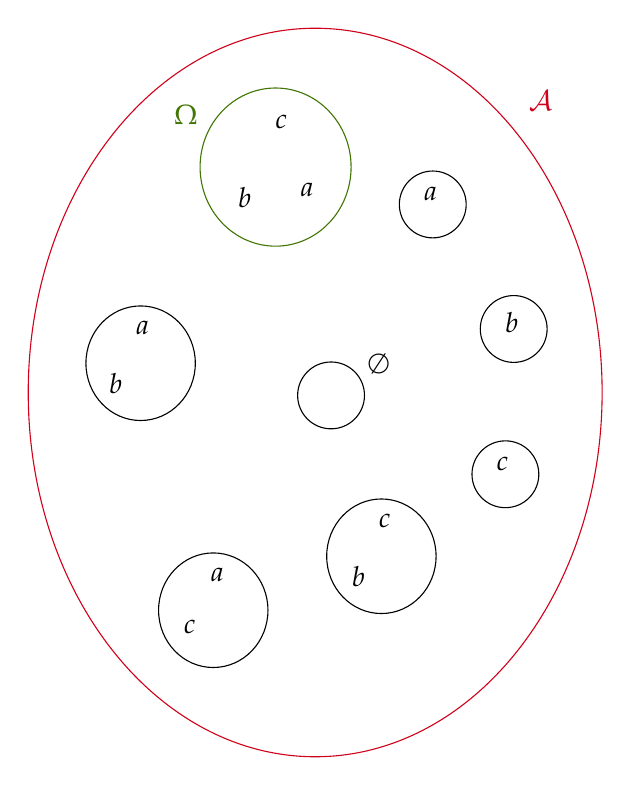
\begin{tikzpicture}[x=0.75pt,y=0.75pt,yscale=-1,xscale=1]
%uncomment if require: \path (0,379); %set diagram left start at 0, and has height of 379

%Shape: Ellipse [id:dp7098699948138527] 
\draw  [color={rgb, 255:red, 208; green, 2; blue, 27 }  ,draw opacity=1 ] (100,182.7) .. controls (100,85.77) and (161.9,7.2) .. (238.25,7.2) .. controls (314.6,7.2) and (376.5,85.77) .. (376.5,182.7) .. controls (376.5,279.63) and (314.6,358.2) .. (238.25,358.2) .. controls (161.9,358.2) and (100,279.63) .. (100,182.7) -- cycle ;
%Shape: Circle [id:dp5932459553762595] 
\draw   (278.8,92.1) .. controls (278.8,83.21) and (286.01,76) .. (294.9,76) .. controls (303.79,76) and (311,83.21) .. (311,92.1) .. controls (311,100.99) and (303.79,108.2) .. (294.9,108.2) .. controls (286.01,108.2) and (278.8,100.99) .. (278.8,92.1) -- cycle ;
%Shape: Circle [id:dp5490421677451254] 
\draw   (317.8,152.1) .. controls (317.8,143.21) and (325.01,136) .. (333.9,136) .. controls (342.79,136) and (350,143.21) .. (350,152.1) .. controls (350,160.99) and (342.79,168.2) .. (333.9,168.2) .. controls (325.01,168.2) and (317.8,160.99) .. (317.8,152.1) -- cycle ;
%Shape: Circle [id:dp31015716407092975] 
\draw   (313.8,222.1) .. controls (313.8,213.21) and (321.01,206) .. (329.9,206) .. controls (338.79,206) and (346,213.21) .. (346,222.1) .. controls (346,230.99) and (338.79,238.2) .. (329.9,238.2) .. controls (321.01,238.2) and (313.8,230.99) .. (313.8,222.1) -- cycle ;
%Shape: Ellipse [id:dp6216043390400294] 
\draw   (127.8,168.6) .. controls (127.8,153.36) and (139.6,141) .. (154.15,141) .. controls (168.7,141) and (180.5,153.36) .. (180.5,168.6) .. controls (180.5,183.84) and (168.7,196.2) .. (154.15,196.2) .. controls (139.6,196.2) and (127.8,183.84) .. (127.8,168.6) -- cycle ;
%Shape: Ellipse [id:dp34537151087018025] 
\draw   (162.8,287.6) .. controls (162.8,272.36) and (174.6,260) .. (189.15,260) .. controls (203.7,260) and (215.5,272.36) .. (215.5,287.6) .. controls (215.5,302.84) and (203.7,315.2) .. (189.15,315.2) .. controls (174.6,315.2) and (162.8,302.84) .. (162.8,287.6) -- cycle ;
%Shape: Ellipse [id:dp9504044872024426] 
\draw   (243.8,261.6) .. controls (243.8,246.36) and (255.6,234) .. (270.15,234) .. controls (284.7,234) and (296.5,246.36) .. (296.5,261.6) .. controls (296.5,276.84) and (284.7,289.2) .. (270.15,289.2) .. controls (255.6,289.2) and (243.8,276.84) .. (243.8,261.6) -- cycle ;
%Shape: Ellipse [id:dp7778615271088332] 
\draw  [color={rgb, 255:red, 65; green, 117; blue, 5 }  ,draw opacity=1 ] (182.8,74.1) .. controls (182.8,53.06) and (199.09,36) .. (219.17,36) .. controls (239.26,36) and (255.55,53.06) .. (255.55,74.1) .. controls (255.55,95.14) and (239.26,112.2) .. (219.17,112.2) .. controls (199.09,112.2) and (182.8,95.14) .. (182.8,74.1) -- cycle ;
%Shape: Circle [id:dp6878415033970087] 
\draw   (229.8,184.1) .. controls (229.8,175.21) and (237.01,168) .. (245.9,168) .. controls (254.79,168) and (262,175.21) .. (262,184.1) .. controls (262,192.99) and (254.79,200.2) .. (245.9,200.2) .. controls (237.01,200.2) and (229.8,192.99) .. (229.8,184.1) -- cycle ;

% Text Node
\draw (340,36) node [anchor=north west][inner sep=0.75pt]  [color={rgb, 255:red, 208; green, 2; blue, 27 }  ,opacity=1 ] [align=left] {$\displaystyle \mathcal{A}$};
% Text Node
\draw (169,43) node [anchor=north west][inner sep=0.75pt]  [color={rgb, 255:red, 65; green, 117; blue, 5 }  ,opacity=1 ] [align=left] {$\displaystyle \Omega $};
% Text Node
\draw (289.4,82.6) node [anchor=north west][inner sep=0.75pt]   [align=left] {$\displaystyle a$};
% Text Node
\draw (328.4,142.6) node [anchor=north west][inner sep=0.75pt]   [align=left] {$\displaystyle b$};
% Text Node
\draw (324.4,212.6) node [anchor=north west][inner sep=0.75pt]   [align=left] {$\displaystyle c$};
% Text Node
\draw (150.65,147.1) node [anchor=north west][inner sep=0.75pt]   [align=left] {$\displaystyle a$};
% Text Node
\draw (137.65,172.1) node [anchor=north west][inner sep=0.75pt]   [align=left] {$\displaystyle b$};
% Text Node
\draw (186.65,266.1) node [anchor=north west][inner sep=0.75pt]   [align=left] {$\displaystyle a$};
% Text Node
\draw (173.65,291.1) node [anchor=north west][inner sep=0.75pt]   [align=left] {$\displaystyle c$};
% Text Node
\draw (267.65,240.1) node [anchor=north west][inner sep=0.75pt]   [align=left] {$\displaystyle c$};
% Text Node
\draw (254.65,265.1) node [anchor=north west][inner sep=0.75pt]   [align=left] {$\displaystyle b$};
% Text Node
\draw (217.82,48.03) node [anchor=north west][inner sep=0.75pt]   [align=left] {$\displaystyle c$};
% Text Node
\draw (199.87,82.55) node [anchor=north west][inner sep=0.75pt]   [align=left] {$\displaystyle b$};
% Text Node
\draw (229.87,80.55) node [anchor=north west][inner sep=0.75pt]   [align=left] {$\displaystyle a$};
% Text Node
\draw (262.4,162.6) node [anchor=north west][inner sep=0.75pt]   [align=left] {$\displaystyle \emptyset $};
\end{tikzpicture}
\end{center}
On peut donc visualiser les 3 conditions dans la définition de la tribu. L'ensemble $\Omega$ est contenu, tous les événements possibles (alias toutes les combinaisons de $\{a, b, c\}$ possibles) sont contenus et tous leurs compléments sont contenus. Finalement, toute union d'événements sera contenue dans la tribu !
\end{formula}




\begin{definitionNOHFILLprop}[Propriétés de la tribu]
Soit $\mathcal{A}$ une tribu sur $\Omega$. Alors : 
\begin{enumerate}[label = \alph*)]
	\item	\lfbox[formula]{$\emptyset \in \mathcal{A}$}.
	\item	$\forall A_{1}, \dots, A_{k} \in \mathcal{A}$, alors \lfbox[formula]{$\displaystyle \bigcup_{i = 1}^{k} A_{i} \in \mathcal{A}$} et \lfbox[formula]{$\displaystyle \bigcap_{i = 1}^{k} A_{i} \in \mathcal{A}$}.
	\item	$\forall (A_{n})_{n \in \mathbb{N}^{\ast}}$ suite d'événements de $\mathcal{A}$, alors \lfbox[formula]{$\displaystyle \bigcap_{n \in \mathbb{N}^{\ast}} A_{n} \in \mathcal{A}$}.
	\item	$\forall (A_{n})_{n \in \mathbb{N}^{\ast}}$ suite d'événements de $\mathcal{A}$, alors \lfbox[formula]{$\lim \inf A_{ n} \in \mathcal{A}$}.
	\item	$\forall (A_{n})_{n \in \mathbb{N}^{\ast}}$ suite d'événements de $\mathcal{A}$, alors \lfbox[formula]{$\lim \sup A_{n} \in \mathcal{A}$}.
\end{enumerate}

\paragraph{Note}	Voir la page 19 des notes de cours du chapitre 1 pour les preuves.
\end{definitionNOHFILLprop}



\columnbreak
\section{Variables aléatoires}
%\begin{rappel_enhanced}[Contexte]
%Souvent, un événement s'énonce de façon numérique (p. ex. : \og rouler un 5 \fg{}, \og pluie de 2mm \fg{}, etc.). Donc, à toute expérience $\omega$, on associe un nombre $X(\omega)$ (ou un $n$-uple de nombres $(X_{1}(\omega), \dots, X_{n}(\omega))$) mesurant un caractère (ou un ensemble de $n$ caractères) du résultat de l'expérience. 
%\end{rappel_enhanced}

\begin{definitionNOHFILL}[Variable aléatoire]
On définit une \textbf{variable aléatoire} comme une \textit{fonction mesurable}. Pour ce faire, on défini 2 espaces mesurables : 
\begin{enumerate}
	\item	On pose que le premier est $(\Omega, \mathcal{A})$.
	\item	On pose que le deuxième est tout ensemble $E$ et sa tribu $\mathcal{E}$ : $(E, \mathcal{E})$.
		\begin{itemize}
		\item	Habituellement, on pose que $E = \mathbb{R}$ et que $\mathcal{E} = \mathcal{B}(\mathbb{R})$.
		\end{itemize}
\end{enumerate}

\bigskip

Une fonction mesurable est une fonction qui associe les éléments de $\Omega$ aux éléments de $E$ avec quelques propriétés additionnelles. On note qu'en associant les éléments de $\Omega$, la fonction associe les \textit{\textbf{éventualités}} et non les \textit{événements} aux éléments de $E$.

\bigskip

On désire avoir une correspondance entre les événements réalisés de $\mathcal{A}$ et l'ensemble transformé d'événements $\mathcal{E}$. Pour ce faire, on impose que la variable aléatoire (alias, la fonction mesurable) $X: \Omega \rightarrow E$ est définie telle que l'image réciproque $X^{-1}(B)$ sur $\Omega$ de tout ensemble $B \in \mathcal{E}$ sur $E$ : \lfbox[formula]{$X^{-1}(B) = \{\omega \in \Omega : X(\omega) \in B\} \in \mathcal{A}$, $\forall B \in \mathcal{E}$}.

\bigskip

Donc, une \textbf{variable aléatoire réelle} est toute application à valeurs réelles $X: \Omega \rightarrow \mathbb{R}$ telle que, $\forall$ intervalle $B$ de $\mathbb{R}$, $\{X \in B\} = X^{-1}(B)$ soit un événement de la tribu $\mathcal{A}$.
\end{definitionNOHFILL}

\begin{formula}{Visualisation}
On peut visualiser que l'événement $B$, où $B \in \mathcal{E}$, a un réciproque $X^{-1}(B)$ où $X^{-1}(B) \in \mathcal{A}$.
\begin{center}
\tikzset{every picture/.style={line width=0.75pt}} %set default line width to 0.75pt        
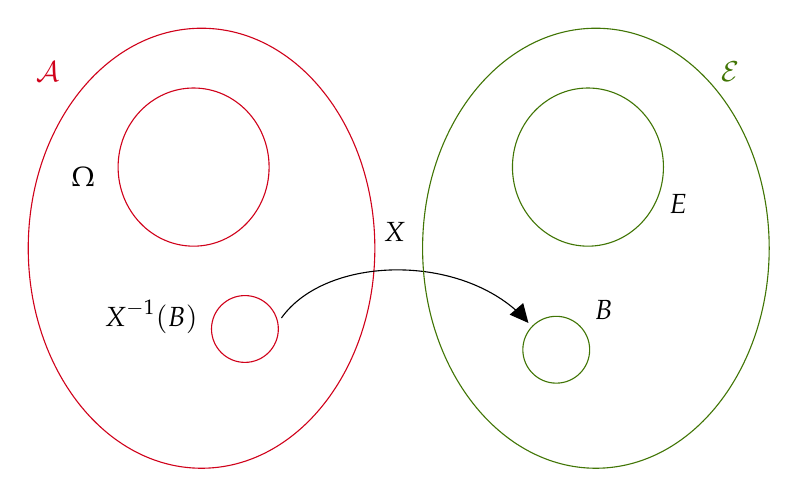
\begin{tikzpicture}[x=0.75pt,y=0.75pt,yscale=-1,xscale=1]
%uncomment if require: \path (0,379); %set diagram left start at 0, and has height of 379

%Shape: Ellipse [id:dp41911676863951963] 
\draw  [color={rgb, 255:red, 208; green, 2; blue, 27 }  ,draw opacity=1 ] (99.5,113.2) .. controls (99.5,54.66) and (136.88,7.2) .. (183,7.2) .. controls (229.12,7.2) and (266.5,54.66) .. (266.5,113.2) .. controls (266.5,171.74) and (229.12,219.2) .. (183,219.2) .. controls (136.88,219.2) and (99.5,171.74) .. (99.5,113.2) -- cycle ;
%Shape: Circle [id:dp8544111010526458] 
\draw  [color={rgb, 255:red, 208; green, 2; blue, 27 }  ,draw opacity=1 ] (187.8,152.1) .. controls (187.8,143.21) and (195.01,136) .. (203.9,136) .. controls (212.79,136) and (220,143.21) .. (220,152.1) .. controls (220,160.99) and (212.79,168.2) .. (203.9,168.2) .. controls (195.01,168.2) and (187.8,160.99) .. (187.8,152.1) -- cycle ;
%Shape: Ellipse [id:dp9026039051255412] 
\draw  [color={rgb, 255:red, 208; green, 2; blue, 27 }  ,draw opacity=1 ] (142.8,74.1) .. controls (142.8,53.06) and (159.09,36) .. (179.17,36) .. controls (199.26,36) and (215.55,53.06) .. (215.55,74.1) .. controls (215.55,95.14) and (199.26,112.2) .. (179.17,112.2) .. controls (159.09,112.2) and (142.8,95.14) .. (142.8,74.1) -- cycle ;
%Curve Lines [id:da98017792051424] 
\draw    (221.5,146.8) .. controls (243.06,116.42) and (308.8,115.24) .. (338.71,147.2) ;
\draw [shift={(340.5,149.2)}, rotate = 229.54] [fill={rgb, 255:red, 0; green, 0; blue, 0 }  ][line width=0.08]  [draw opacity=0] (8.93,-4.29) -- (0,0) -- (8.93,4.29) -- cycle    ;
%Shape: Ellipse [id:dp40560748374308386] 
\draw  [color={rgb, 255:red, 65; green, 117; blue, 5 }  ,draw opacity=1 ] (289.5,113.2) .. controls (289.5,54.66) and (326.88,7.2) .. (373,7.2) .. controls (419.12,7.2) and (456.5,54.66) .. (456.5,113.2) .. controls (456.5,171.74) and (419.12,219.2) .. (373,219.2) .. controls (326.88,219.2) and (289.5,171.74) .. (289.5,113.2) -- cycle ;
%Shape: Circle [id:dp12681144619815132] 
\draw  [color={rgb, 255:red, 65; green, 117; blue, 5 }  ,draw opacity=1 ] (337.8,162.1) .. controls (337.8,153.21) and (345.01,146) .. (353.9,146) .. controls (362.79,146) and (370,153.21) .. (370,162.1) .. controls (370,170.99) and (362.79,178.2) .. (353.9,178.2) .. controls (345.01,178.2) and (337.8,170.99) .. (337.8,162.1) -- cycle ;
%Shape: Ellipse [id:dp4643784990820654] 
\draw  [color={rgb, 255:red, 65; green, 117; blue, 5 }  ,draw opacity=1 ] (332.8,74.1) .. controls (332.8,53.06) and (349.09,36) .. (369.17,36) .. controls (389.26,36) and (405.55,53.06) .. (405.55,74.1) .. controls (405.55,95.14) and (389.26,112.2) .. (369.17,112.2) .. controls (349.09,112.2) and (332.8,95.14) .. (332.8,74.1) -- cycle ;

% Text Node
\draw (102,22) node [anchor=north west][inner sep=0.75pt]  [color={rgb, 255:red, 208; green, 2; blue, 27 }  ,opacity=1 ] [align=left] {$\displaystyle \mathcal{A}$};
% Text Node
\draw (119,73) node [anchor=north west][inner sep=0.75pt]  [color={rgb, 255:red, 0; green, 0; blue, 0 }  ,opacity=1 ] [align=left] {$\displaystyle \Omega $};
% Text Node
\draw (135,137) node [anchor=north west][inner sep=0.75pt]  [color={rgb, 255:red, 0; green, 0; blue, 0 }  ,opacity=1 ] [align=left] {$\displaystyle X^{-1}( B)$};
% Text Node
\draw (269.4,99.6) node [anchor=north west][inner sep=0.75pt]   [align=left] {$\displaystyle X$};
% Text Node
\draw (432,22) node [anchor=north west][inner sep=0.75pt]  [color={rgb, 255:red, 65; green, 117; blue, 5 }  ,opacity=1 ] [align=left] {$\displaystyle \mathcal{E}$};
% Text Node
\draw (407,86) node [anchor=north west][inner sep=0.75pt]  [color={rgb, 255:red, 0; green, 0; blue, 0 }  ,opacity=1 ] [align=left] {$\displaystyle E$};
% Text Node
\draw (371,137) node [anchor=north west][inner sep=0.75pt]  [color={rgb, 255:red, 0; green, 0; blue, 0 }  ,opacity=1 ] [align=left] {$\displaystyle B$};
\end{tikzpicture}
\end{center}
\end{formula}

\bigskip

En posant $E = \mathbb{R}$ et $\mathcal{E} = \mathcal{B}(\mathbb{R})$, on obtient la \textit{tribu borélienne}.
\begin{definitionNOHFILLsub}[Tribu borélienne]
La tribu borélienne $\mathcal{B}_{\mathbb{R}}$ est la plus petite tribu de $\mathbb{R}$ qui contient tous ses intervalles. Les éléments de $\mathcal{B}_{\mathbb{R}}$ sont appelés les \textbf{\textit{boréliens}} de $\mathbb{R}$.

\bigskip

Pour une v.a. réelle $X$, $\forall B \in \mathcal{B}_{\mathbb{R}}$ on a $X^{-1}(B) \in \mathcal{A}$. 

\bigskip

Bref, \lfbox[formula]{$(\Omega, \mathcal{A}) \overset{X}{\rightarrow} (\mathbb{R}, \mathcal{B}_{\mathbb{R}})$}. On dit que la tribu $X^{-1}(\mathcal{B}_{\mathbb{R}})$ sur $\Omega$ est la \textbf{\textit{tribu des événements engendrés par $X$}}.
\end{definitionNOHFILLsub}



\columnbreak
\section{Probabilités}
\begin{definitionNOHFILL}[Mesure]
Pour un espace mesurable $(\Omega, \mathcal{A})$, une fonction \lfbox[formula]{$\mathbb{P}: \mathcal{A} \rightarrow [0, \infty]$} s'appelle une \textbf{mesure} sur $(\Omega, \mathcal{A})$ si :
\begin{enumerate}
	\item	Elle attribue une masse de zéro à l'ensemble vide : \lfbox[conditions]{$\mathbb{P}(\emptyset) = 0$}.
	\item	Elle est \og \textit{countably additive} \fg{} : \lfbox[conditions]{$\displaystyle P\left(\bigcup_{i} A_{i}\right) = \sum_{i} P(A_{i})$, $\forall A_{i} \in \mathcal{A}$}.
\end{enumerate}
\end{definitionNOHFILL}


\begin{definitionNOHFILLsub}[Mesure de probabilité]
Pour un espace probabilisable $(\Omega, \mathcal{A})$, on appelle \textbf{\textit{probabilité}} sur $(\Omega, \mathcal{A})$ toute \underline{application} $P: \mathcal{A} \rightarrow [0, 1]$ telle que :
\begin{enumerate}[label = \roman*)]
	\item	\lfbox[conditions]{$P(\Omega) = 1$}.
	\item	$\forall (A_{n})_{n \in \mathbb{N}^{\ast}}$ d'événements deux à deux disjoints, \lfbox[conditions]{$\displaystyle P\left(\bigcup_{n \in \mathbb{N}^{\ast}} A_{n}\right) = \sum_{n \in \mathbb{N}^{\ast}} P(A_{n})$}.
\end{enumerate}

\bigskip

La mesure de probabilité est donc une mesure qui est \textbf{restreint} sur $[0, 1]$.
\end{definitionNOHFILLsub}

\begin{definitionNOHFILL}[Espace probabilisé]
Le triplet $(\Omega, \mathcal{A}, P)$ s'appelle un \textbf{espace probabilisé} et est composé de : 
\begin{description}
	\item[$\Omega$]	Le \og \textit{sample space} \fg{}.
	\item[$\mathcal{A}$]	Le \og \textit{event space} \fg{}.
	\item[$P$]	La \textbf{\textit{mesure} de probabilité}.
\end{description}

\begin{itemize}
	\item	En anglais, on dit \og \textit{\textbf{probability space}} \fg{}.
\end{itemize}
\end{definitionNOHFILL}

\begin{formula}{Visualisation}
Voici une visualisation de ce que représente l'\textit{application} $P$ : 
\begin{center}
\tikzset{every picture/.style={line width=0.75pt}} %set default line width to 0.75pt        
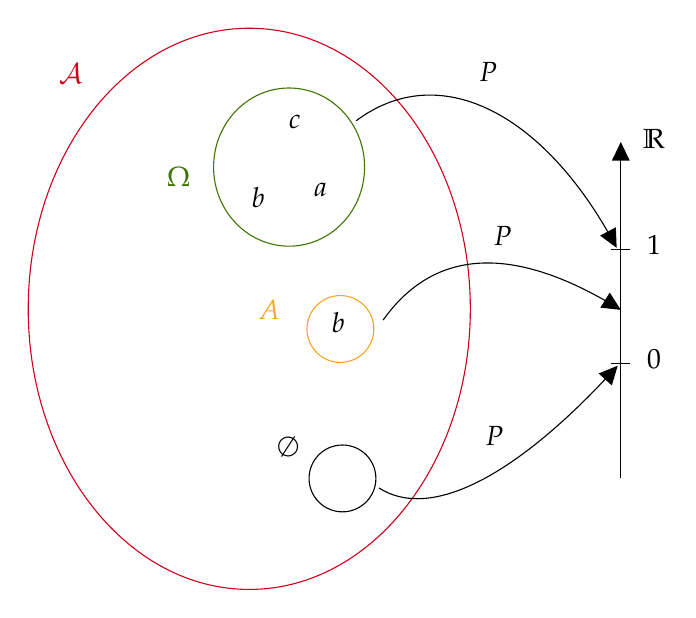
\begin{tikzpicture}[x=0.75pt,y=0.75pt,yscale=-1,xscale=1]
%uncomment if require: \path (0,379); %set diagram left start at 0, and has height of 379

%Shape: Ellipse [id:dp7275335040924429] 
\draw  [color={rgb, 255:red, 208; green, 2; blue, 27 }  ,draw opacity=1 ] (143.5,142.4) .. controls (143.5,67.73) and (191.18,7.2) .. (250,7.2) .. controls (308.82,7.2) and (356.5,67.73) .. (356.5,142.4) .. controls (356.5,217.06) and (308.82,277.59) .. (250,277.59) .. controls (191.18,277.59) and (143.5,217.06) .. (143.5,142.4) -- cycle ;
%Shape: Circle [id:dp7731815975229219] 
\draw  [color={rgb, 255:red, 245; green, 166; blue, 35 }  ,draw opacity=1 ] (277.8,152.1) .. controls (277.8,143.21) and (285.01,136) .. (293.9,136) .. controls (302.79,136) and (310,143.21) .. (310,152.1) .. controls (310,160.99) and (302.79,168.2) .. (293.9,168.2) .. controls (285.01,168.2) and (277.8,160.99) .. (277.8,152.1) -- cycle ;
%Shape: Ellipse [id:dp05212878447489011] 
\draw  [color={rgb, 255:red, 65; green, 117; blue, 5 }  ,draw opacity=1 ] (232.8,74.1) .. controls (232.8,53.06) and (249.09,36) .. (269.17,36) .. controls (289.26,36) and (305.55,53.06) .. (305.55,74.1) .. controls (305.55,95.14) and (289.26,112.2) .. (269.17,112.2) .. controls (249.09,112.2) and (232.8,95.14) .. (232.8,74.1) -- cycle ;
%Shape: Circle [id:dp7692168919967604] 
\draw   (278.8,224.1) .. controls (278.8,215.21) and (286.01,208) .. (294.9,208) .. controls (303.79,208) and (311,215.21) .. (311,224.1) .. controls (311,232.99) and (303.79,240.2) .. (294.9,240.2) .. controls (286.01,240.2) and (278.8,232.99) .. (278.8,224.1) -- cycle ;
%Straight Lines [id:da2483716446626154] 
\draw    (429,223.8) -- (429,65) (424.5,168.8) -- (433.5,168.8)(424.5,113.8) -- (433.5,113.8) ;
\draw [shift={(429,62)}, rotate = 450] [fill={rgb, 255:red, 0; green, 0; blue, 0 }  ][line width=0.08]  [draw opacity=0] (8.93,-4.29) -- (0,0) -- (8.93,4.29) -- cycle    ;
%Curve Lines [id:da9846347851794925] 
\draw    (301.5,51.8) .. controls (341.1,22.1) and (391.48,47.29) .. (425.96,111.06) ;
\draw [shift={(427,113)}, rotate = 242.11] [fill={rgb, 255:red, 0; green, 0; blue, 0 }  ][line width=0.08]  [draw opacity=0] (8.93,-4.29) -- (0,0) -- (8.93,4.29) -- cycle    ;
%Curve Lines [id:da7092634548038517] 
\draw    (314.5,147.8) .. controls (336.17,117.27) and (371.42,108.07) .. (426.47,141.35) ;
\draw [shift={(429,142.9)}, rotate = 211.85] [fill={rgb, 255:red, 0; green, 0; blue, 0 }  ][line width=0.08]  [draw opacity=0] (8.93,-4.29) -- (0,0) -- (8.93,4.29) -- cycle    ;
%Curve Lines [id:da838947272903674] 
\draw    (312.5,228.7) .. controls (337.25,244.64) and (378.66,223.24) .. (426.06,171.38) ;
\draw [shift={(427.5,169.8)}, rotate = 492.17] [fill={rgb, 255:red, 0; green, 0; blue, 0 }  ][line width=0.08]  [draw opacity=0] (8.93,-4.29) -- (0,0) -- (8.93,4.29) -- cycle    ;

% Text Node
\draw (157,23) node [anchor=north west][inner sep=0.75pt]  [color={rgb, 255:red, 208; green, 2; blue, 27 }  ,opacity=1 ] [align=left] {$\displaystyle \mathcal{A}$};
% Text Node
\draw (209,73) node [anchor=north west][inner sep=0.75pt]  [color={rgb, 255:red, 65; green, 117; blue, 5 }  ,opacity=1 ] [align=left] {$\displaystyle \Omega $};
% Text Node
\draw (288.4,142.6) node [anchor=north west][inner sep=0.75pt]   [align=left] {$\displaystyle b$};
% Text Node
\draw (267.82,48.03) node [anchor=north west][inner sep=0.75pt]   [align=left] {$\displaystyle c$};
% Text Node
\draw (249.87,82.55) node [anchor=north west][inner sep=0.75pt]   [align=left] {$\displaystyle b$};
% Text Node
\draw (279.87,80.55) node [anchor=north west][inner sep=0.75pt]   [align=left] {$\displaystyle a$};
% Text Node
\draw (262.4,202.6) node [anchor=north west][inner sep=0.75pt]   [align=left] {$\displaystyle \emptyset $};
% Text Node
\draw (253,137) node [anchor=north west][inner sep=0.75pt]  [color={rgb, 255:red, 245; green, 166; blue, 35 }  ,opacity=1 ] [align=left] {$\displaystyle A$};
% Text Node
\draw (438.4,54.6) node [anchor=north west][inner sep=0.75pt]   [align=left] {$\displaystyle \mathbb{R}$};
% Text Node
\draw (440.4,105.6) node [anchor=north west][inner sep=0.75pt]   [align=left] {$\displaystyle 1$};
% Text Node
\draw (440.4,160.6) node [anchor=north west][inner sep=0.75pt]   [align=left] {$\displaystyle 0$};
% Text Node
\draw (359.4,22.6) node [anchor=north west][inner sep=0.75pt]   [align=left] {$\displaystyle P$};
% Text Node
\draw (366.4,101.6) node [anchor=north west][inner sep=0.75pt]   [align=left] {$\displaystyle P$};
% Text Node
\draw (362.4,197.6) node [anchor=north west][inner sep=0.75pt]   [align=left] {$\displaystyle P$};
\end{tikzpicture}
\end{center}
On peut donc visualiser les 2 conditions dans la définition de l'espace probabilisé. La probabilité d'observer l'ensemble $\Omega$ est de $1$ car il contient tous les événements possibles. La probabilité d'un événement sera contenu entre $0$ et $1$ ce qui veut dire que la probabilité de quelques événements \textit{disjoints} correspond à la somme des probabilités. 
\end{formula}

On complète la notion précédente sur l'espace borélien avec $(\Omega, \mathcal{A}, P) \overset{X}{\rightarrow} (\mathbb{R}, \mathcal{B}_{\mathbb{R}}, P_{X})$ où $P_{X}$ est appelée loi de probabilité de $X$. On définit $P_{X}(B) = P(X \in B) = P\left(X^{-1}(B)\right)$.


\begin{definitionNOHFILLprop}[Propriétés des probabilités]
Soit $(\Omega, \mathcal{A}, P)$ un espace probabilisé. Alors : 
\begin{enumerate}[label = \alph*)]
	\item	$P(\emptyset) = 0$.
	\item	Si $A$ et $B$ sont des événements disjoints, alors \lfbox[formula]{$P(A \cup B) = P(A) + P(B)$}.
	\item	Si $A$ et $B$ sont des événements quelconques, alors \lfbox[formula]{$P(A \cup B) = P(A) + P(B) - P(A \cap B)$}.
	\item	Si $A$ et $B$ sont des événements tels que $A \subset B$, alors \lfbox[formula]{$P(B \smallsetminus A) = P(B) - P(A)$} et \lfbox[formula]{$P(A) \leq P(B)$}.
	\item	$\forall A \in \mathcal{A}$, \lfbox[formula]{$P(A^{c}) = 1 - P(A)$}.
	\item	Si $(A_{n})_{n \in \mathbb{N}^{\ast}}$ est une suite d'événements quelconques, alors \lfbox[formula]{$\displaystyle P\left(\bigcup_{n \in \mathbb{N}^{\ast}} A_{n}\right) \leq \sum_{n \in \mathbb{N}^{\ast}} P(A_{n})$}.
	\item	Si $(A_{n})_{n \in \mathbb{N}^{\ast}}$ est une suite d'événements tels que $A_{n} \downarrow \emptyset$, alors \lfbox[formula]{$P(A_{n}) \downarrow 0$}.
	\item	Si $(A_{n})_{n \in \mathbb{N}^{\ast}}$ est une suite d'événements tels que $A_{n} \downarrow A$, alors \lfbox[formula]{$P(A_{n}) \downarrow P(A)$}.
	\item	Si $(A_{n})_{n \in \mathbb{N}^{\ast}}$ est une suite d'événements tels que $A_{n} \uparrow A$, alors \lfbox[formula]{$P(A_{n}) \uparrow P(A)$}.
\end{enumerate}
\end{definitionNOHFILLprop}



\columnbreak
\section{Lemmes de Borel-Cantelli}
\begin{definitionNOHFILL}[Lemme de Borel-Cantelli \textit{(1ère partie)}]
Si $(A_{n})_{n \in \mathbb{N}^{\ast}}$ est une suite d'événements telle que : \lfbox[conditions]{$\displaystyle \sum_{n = 1}^{\infty} P(A_{n}) < \infty$}, alors \lfbox[formula]{$\displaystyle P\left(\limsup_{n \rightarrow \infty} A_{n}\right) = 0$}.
\end{definitionNOHFILL}



\subsection{Probabilité conditionnelle}
\begin{definitionNOHFILLpropos}[Formule de Bayes \textit{(2 événements)}]
Soit un espace probabilisé $(\Omega, \mathcal{A}, P)$, $A$ et $B$ deux événements de $\mathcal{A}$ tels que $\Pr(A) \neq 0$, $\Pr(A^{C}) \neq 0$  et $\Pr(B) \neq 0$. Alors : 
\begin{align*}
	\Pr(A \smallsetminus B)
	&=	\frac{\Pr(B | A)\Pr(A)}{\Pr(B | A)\Pr(A) + \Pr(B | A^{C})\Pr(A^{C})}
\end{align*}
\end{definitionNOHFILLpropos}


\begin{definitionNOHFILLpropos}[Théorème des probabilités totales]
Soit un espace probabilisé $(\Omega, \mathcal{A}, P)$ et $(A_{i})_{i \in \mathbb{N}}$ une partition de $\Omega$ telle que $\forall i$, $\Pr(A_{i}) \neq 0$. Alors, $\forall B \in \mathcal{A}$, \lfbox[formula]{$\displaystyle \Pr(B) = \sum_{i \in \mathbb{N}}\Pr(B | A_{i})\Pr(A_{i})$}.

\end{definitionNOHFILLpropos}
\begin{definitionNOHFILLpropos}[Formule de Bayes \textit{($n$ événements)}]
Soit un espace probabilisé $(\Omega, \mathcal{A}, P)$ et $(A_{i})_{i = 1, 2, \dots, n}$ une partition \textbf{finie} de $\Omega$ telle que $\forall i$, $\Pr(A_{i}) \neq 0$. Alors, $\forall B \in \mathcal{A}$ tel que $\Pr(B) \neq 0$,
\begin{align*}
	\Pr(A_{i} | B)
	&=	\frac{\Pr(B | A_{i})\Pr(A_{i})}{\sum_{j = 1}^{n} \Pr(B | A_{j})\Pr(A_{j})}
\end{align*}
\end{definitionNOHFILLpropos}


\columnbreak
\subsection{Indépendance}
\begin{definitionNOHFILL}[Indépendance \textit{(2 événements)}]
Soit un espace probabilisé $(\Omega, \mathcal{A}, P)$, $A$ et $B$ deux événements de $\mathcal{A}$. Alors $A$ et $B$ sont indépendants \underline{pour la probabilité $P$} \textbf{\underline{si et seulement si}} \lfbox[formula]{$\Pr(A \cap B) = \Pr(A) \Pr(B)$}.

\bigskip

Il est important de bien saisir que le notion d'indépendance n'est pas intrinsèque aux événements, mais \textit{dépend} de la probabilité $P$ choisie sur $(\Omega, \mathcal{A})$. Deux événements peuvent êtres indépendants pour une probabilité, \underline{mais être dépendants pour une autre}.

\bigskip

\begin{definitionNOHFILLprop}[Propriétés \textit{(2 événements)}]
\begin{enumerate}[label = \rectangled{\arabic*}{lightgray}]
	\item	$A^{C}$ et $B$ sont indépendants.
	\item	$A$ et $B^{C}$ sont indépendants.
	\item	$A^{C}$ et $B^{C}$ sont indépendants.
\end{enumerate}
\end{definitionNOHFILLprop}
\end{definitionNOHFILL}

\begin{definitionNOHFILL}[Indépendance \textit{($n$ événements)}]
Soient $(A_{1}, \dots, A_{n})$ un $n$-uple d'événements. On dit qu'ils sont \textbf{indépendants}, ou \textbf{\textit{mutuellement indépendants}}, \underline{\textbf{si et seulement si}} $\forall k = 1, \dots, n$, si $\forall$ sous-ensemble $(A_{i_{1}}, \dots, A_{i_{k}})$ de $k$ événements choisis parmi les $(A_{1}, \dots, A_{n})$, on a \lfbox[formula]{$\Pr(A_{i_{1}} \cap \dots \cap A_{i_{k}}) = \Pr(A_{i_{1}}) \times \cdot \times \Pr(A_{i_{k}})$}.
\end{definitionNOHFILL}

\begin{definitionNOHFILL}[Indépendance \textit{(suite d'événements)}]
Soit un espace probabilisé $(\Omega, \mathcal{A}, P)$, et une suite d'événements indépendants $(A_{n})_{n \in \mathbb{N}^{\ast}}$ de $\mathcal{A}$. Alors on a \lfbox[formula]{$\displaystyle \Pr\left(\bigcap_{n \in \mathbb{N}^{\ast}} A_{n}\right) = \lim_{k \rightarrow \infty} \prod_{n = 1}^{k} \Pr(A_{n})$}.
\end{definitionNOHFILL}


\begin{definitionNOHFILL}[Lemme de Borel-Cantelli (2ème partie)]
Soit $(\Omega, \mathcal{A}, P)$ un espace probabilisé, et une suite d'événements $(A_{n})_{n \in \mathbb{N}^{\ast}}$ indépendants de $\mathcal{A}$ telle que \lfbox[conditions]{$\displaystyle \sum_{n = 1}^{\infty} \Pr(A_{n}) = \infty$}, alors \lfbox[formula]{$\Pr\left(\limsup_{n} A_{n}\right) = 1$}
\end{definitionNOHFILL}



\columnbreak
\section{Fonction de répartition}
\begin{definitionNOHFILL}[Mesure image]
La mesure image, ou \og \textit{pushforward measure} \fg{} en anglais, est obtenue \og \textit{by pushing} \fg{} une mesure d'un espace mesurable à un autre avec une fonction mesurable.
\end{definitionNOHFILL}

\begin{definitionNOHFILL}[Loi de probabilité]
La \textit{mesure image} de $P$ par $X$, notée \lfbox[formula]{$P_{X}$}, s'appelle la \textbf{\textit{loi de probabilité}} de $X$.
\end{definitionNOHFILL}

\begin{definitionNOHFILLsub}[Fonction de répartition]
Pour une mesure de probabilité $P_{X}$, on a que $\forall x \in \mathbb{R}$ la fonction $F$ est définie comme \lfbox[formula]{$F(x) = P_{X}(]-\infty, x])$}. Cette fonction a les propriétés suivantes : 
\begin{enumerate}[label = \circled{\arabic*}{trueblue}]
	\item	$F$ est croissante au sens large.
	\item	$F$ est continue à droite.
	\item	$\lim_{x \rightarrow \infty} F(x) = 1$ et $\lim_{x \rightarrow -\infty} F(x) = 0$.
\end{enumerate}
\end{definitionNOHFILLsub}

\paragraph{Note}	Il y a une relation biunivoque entre les mesures de probabilités sur $(\mathbb{R}, \mathcal{B}_{\mathbb{R}})$ et les fonctions de répartition.

\bigskip

\subsection{Classification des lois de probabilité sur la tribu borélienne}
Pour une probabilité $P$ sur $(\mathbb{R}, \mathcal{B}_{\mathbb{R}})$, on classifie les lois de probabilités en 2 groupes :
\begin{definitionGENERAL}{Diffuse}[\circled{1}{trueblue}]
On dit que $P$ est diffuse si $\forall x \in \mathbb{R}$, \lfbox[formula]{$P(x) = 0$}.
\end{definitionGENERAL}

\begin{definitionGENERAL}{Discrète}[\circled{2}{trueblue}]
On dit que $P$ est discrète s'il existe un ensemble au plus dénombrable $S$ tel que \lfbox[formula]{$P(S) = 1$}.
\end{definitionGENERAL}

Cependant, si $P$ désigne une probabilité sur $(\mathbb{R}, \mathcal{B}_{\mathbb{R}})$ ni diffuse ni discrète, alors $\exists \alpha \in ]0, 1[$, $P_{1}$ une loi discrète et $P_{2}$ une loi diffuse tel que \lfbox[formula]{$P = \alpha P_{1} + (1 - \alpha)P_{2}$}.

\bigskip

\begin{definitionNOHFILL}[Variable aléatoire discrète]
Toute variable aléatoire $X$ telle qu'il existe un sous-ensemble fini ou dénombrable $S_{X}$ (ou tout simplement $S$) de $\mathbb{R}$ vérifiant $P(\{X \in S\} = 1$. On peut donc définir \lfbox[formula]{$S = \left\{x \in \mathbb{R} : P_{X}(\{x\}) = P((\{X = x\}) > 0\right\}$}. Donc, on note $p_{x} = P((\{X = x\}) = P_{X}(\{x\})$
\end{definitionNOHFILL}

\begin{definitionNOHFILL}[Loi continue]
Une mesure de probabilité absolument continue est une mesure de probabilité de la forme \lfbox[formula]{$P(B) = \int_{B} f(x)dx$} $\forall B \in \mathcal{B}_{\mathbb{R}}$ où $f$ est une densité de probabilité. C'est-à-dire, une fonction définie sur $\mathbb{R}$ satisfaisant aux conditions : 
\begin{enumerate}[label = \circled{\arabic*}{trueblue}]
	\item	$f(x) \geq 0$ $\forall x \in \mathbb{R}$,
	\item	$\int_{-\infty}^{\infty} f(x)dx = 1$
\end{enumerate}

Toute variable aléatoire $X$ telle qu'il existe un sous-ensemble fini ou dénombrable $S_{X}$ (ou tout simplement $S$) de $\mathbb{R}$ vérifiant $P(\{X \in S\} = 1$. On peut donc définir \lfbox[formula]{$S = \left\{x \in \mathbb{R} : P_{X}(\{x\}) = P((\{X = x\}) > 0\right\}$}. Donc, on note $p_{x} = P((\{X = x\}) = P_{X}(\{x\})$
\end{definitionNOHFILL}


\newpage
\chapter{Moments et transformations de variables}
\section{Cas discret}
\begin{definitionNOHFILL}[Espérance]
Sous réserve d'existence, l'\textbf{\textit{espérance mathématique}} ou la \textit{moyenne} de $X$ est le nombre \lfbox[formula]{$\text{E}[X] = m_{X} = \sum_{k} x_{k} P(X = x_{k})$}.

\bigskip

\begin{definitionNOHFILLprop}[Invariance à la translation ou multiplication par un scalaire]
Pour $a, b \in \mathbb{R}$, \lfbox[formula]{$\text{E}[aX + b] = a\text{E}[X] + b$}.
\end{definitionNOHFILLprop}

\begin{definitionNOHFILLprop}[Espérance d'une puissance $s$]
Sous réserve d'existence, \lfbox[formula]{$\text{E}[X^{s}] = \sum_{x \in S}x^{s} P_{X}(x)$}.
\end{definitionNOHFILLprop}
\end{definitionNOHFILL}


\begin{definitionNOHFILL}[Variance]
Sous réserve d'existence, la \textbf{variance} de $X$ est le nombre \lfbox[formula]{$\text{Var}(X)$} ou \lfbox[formula]{$\sigma^{2}_{X}$} où \lfbox[formula]{$\text{Var}(X) = \text{E}\left[\left(X - \text{E}[X]\right)^{2}\right] = \sum_{x \in S} (x - m_{X})^{2} P(X = x)$}. On peut également réécrire \lfbox[formula]{$\text{E}\left[\left(X - \text{E}[X]\right)^{2}\right]  = \text{E}\left[X^{2}\right] - \left(\text{E}[X]\right)^{2}$}.

\bigskip

\begin{definitionNOHFILLprop}[Translation ou multiplication par un scalaire]
Pour $a, b \in \mathbb{R}$, \lfbox[formula]{$\text{Var}(aX + b) = a^{2}\text{Var}(X)$}. Donc, contrairement à l'espérance, la variance n'est \textbf{pas} invariante à la translation ou multiplication par un scalaire.

\end{definitionNOHFILLprop}
\end{definitionNOHFILL}


\begin{definitionNOHFILL}[Moment centré et réduit de puissance $s$]
Sous réserve d'existence, le \textbf{moment centrée $s$} de $X$ est \lfbox[formula]{$\text{E}\left[\left(X - \text{E}[X]\right)^{s}\right]$}.

\begin{definitionNOHFILLsub}[Variable aléatoire réelle centrée]
Sous réserve d'existence de la moyenne, toute variable dont la moyenne est nulle.
\end{definitionNOHFILLsub}
\begin{definitionNOHFILLsub}[Variable aléatoire réelle réduite]
Sous réserve d'existence de la moyenne, toute variable de variance 1.
\end{definitionNOHFILLsub}
Donc, la variable aléatoire réelle \textbf{centrée et réduite} est, sous réserve d'existence, toute variable de moyenne nulle et de variance 1.
\end{definitionNOHFILL}

\bigskip


\begin{definitionNOHFILL}[Covariance]
La covariance entre deux variables $X$ et $Y$ est \lfbox[formula]{$Cov(X, Y) = \text{E}\left[\left(X - \text{E}[X]\right)\left(Y - \text{E}[Y]\right)\right]$}.
\end{definitionNOHFILL}

\subsubsection{Vecteur}
\begin{definitionNOHFILL}[Espérance d'un vecteur]
Soit un vecteur aléatoire de $n$ v.a. discrètes $\bm{X} = (X_{1}, \dots, X_{n})$. Sous réserve d'existence de $\text{E}[X_{i}]$ pour $i = 1, 2, \dots, n$, l'\textbf{espérance mathématique} de $\bm{X}$ est le $n$-uple \lfbox[formula]{$\left(\text{E}[X_{1}], \dots, \text{E}[X_{n}]\right)$}.

\begin{definitionNOHFILLprop}[Espérance de la somme]
Si l'espérance mathématique du vecteur $\bm{X}$ existe, alors l'espérance mathématique de la somme $X_{1} + \cdots + X_{n}$ est \lfbox[formula]{$\text{E}[X_{1} + \cdots + X_{n}] = \text{E}[X_{1}] + \cdots + \text{E}[X_{n}]$}.
\end{definitionNOHFILLprop}

\begin{definitionNOHFILLprop}[Espérance du produit]
Si l'espérance mathématique du vecteur $\bm{X}$ existe, et que les \textbf{composantes du vecteur sont indépendantes}, alors l'espérance mathématique du produit $X_{1} \times \cdots \times X_{n}$ est \lfbox[formula]{$\text{E}[X_{1} \times \cdots \times X_{n}] = \text{E}[X_{1}] \times \cdots \times \text{E}[X_{n}]$}.
\end{definitionNOHFILLprop}
\end{definitionNOHFILL}


\bigskip


\begin{definitionNOHFILL}[Matrice de variances-covariances d'un vecteur]
Si elle existe, la matrice de variances-covariances d'un vecteur aléatoire $(X_{1}, \dots, X_{n})$ est définie par le terme général $\forall i, j$  t.q. $1 \leq i, j \leq n$ : \lfbox[formula]{$Cov(X_{i}, X_{j}) = \text{E}\left[\left(X_{i} - \text{E}[X_{i}]\right)\left(X_{j} - \text{E}[X_{j}]\right)\right]$}.

\bigskip

\begin{definitionNOHFILLprop}[Variance de la somme]
Si le vecteur aléatoire $\bm{X}$ est composé de v.a.r. discrètes \textbf{indépendantes}, dont le moment d'ordre 2 existe, alors la variance de la somme \lfbox[formula]{$\sigma^{2}_{X_{1} + \cdots + X_{n}} = \sigma^{2}_{X_{1}} + \cdots  + \sigma^{2}_{X_{n}}$}.
\end{definitionNOHFILLprop}
\end{definitionNOHFILL}


\subsubsection{Autres mesures}
\begin{definitionNOHFILL}[Coefficient de corrélation de Pearson]
Soit le couple de v.a.r. $(X, Y)$, possédant des variances non nulles, le \textbf{coefficient de corrélation} de $X$ et de $Y$ est le nombre \lfbox[formula]{$\rho(X, Y) = \frac{\text{Cov}(X, Y)}{\sigma_{X}\sigma_{Y}}$}.
\end{definitionNOHFILL}



\columnbreak
\section{Cas continu}


\columnbreak
\section{Lois conditionnelles continues}


\columnbreak
\section{Fonction génératrice des moments}


\columnbreak
\section{Calcul de lois}




\end{multicols*}
\end{document}
